% ==========================================
% step03.tex
% ==========================================
\section{بخش سوم: بهبود جامع کیفیت به کمک انتقال افاین ($a \times I + b$)}

\noindent
استفاده‌ی مجزا از عملگرهای جمع (برای اصلاح روشنایی) و ضرب (برای اصلاح کنتراست) نشان داد که یک عملگر به‌تنهایی نمی‌تواند کیفیت تصویر را به حالت ایده‌آل برساند. در این بخش، عملگر خطی جامع $I' = a \times I + b$ که به انتقال افاین (\lr{Affine Transformation}) معروف است پیاده‌سازی شده است. این عملگر به ما اجازه می‌دهد هیستوگرام را همزمان بسط داده و در مرکز بازه متمرکز کنیم.

\begin{stepbox}
\field{۱. استخراج روابط ریاضی و پیاده‌سازی پارامترهای بهینه}{
هدف ما در این بخش، رسیدن به توزیع نوری متعادل با میانگین ایده‌آل در مرکز بازه ($\mu_{new} = 128$) و انحراف معیار بالا بر اساس قانون $4\sigma$ ($\sigma_{new} = 64$) است. بر اساس قوانین امید ریاضی و واریانس داریم:
\[
\mu_{new} = a \times \mu_{old} + b \quad , \quad \sigma_{new} = a \times \sigma_{old}
\]
با حل این دستگاه معادلات، مقادیر بهینه مستقیماً محاسبه می‌شوند:
\[
a_{opt} = \frac{64}{\sigma_{old}} \quad , \quad b_{opt} = 128 - a_{opt} \times \mu_{old}
\]
}
\end{stepbox}

\begin{codebox}[پیاده‌سازی الگوریتم انتقال افاین]
\begin{lstlisting}[language=Python]
# --- Affine Transformation for Bright/Dark Images ---
I_float = I.astype(np.float32)
mu_old = I_float.mean()
std_old = I_float.std()

# Added epsilon (1e-7) to prevent ZeroDivisionError for uniform images
a_opt = 64 / (std_old + 1e-7)
b_opt = 128 - (a_opt * mu_old)

I_new = (a_opt * I_float) + b_opt
new_image = np.clip(I_new, 0, 255).astype(np.uint8)
\end{lstlisting}
\end{codebox}

\begin{figure}[htbp]
\centering
\begin{subfigure}{0.48\textwidth}
    \centering
    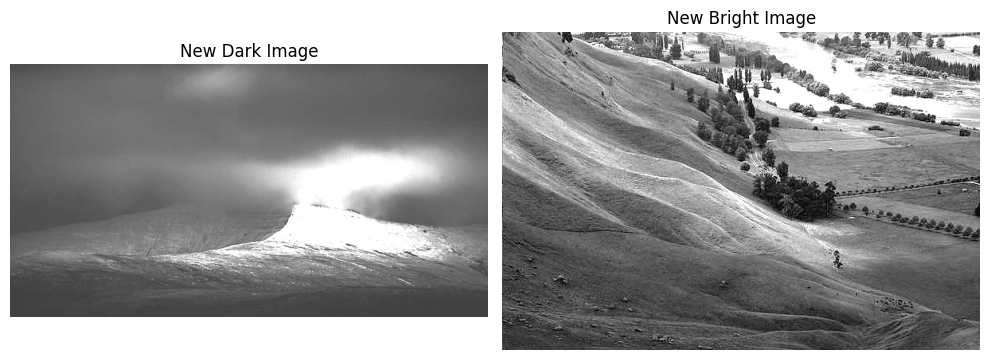
\includegraphics[width=0.9\linewidth]{images/image_2572b4.png} % تصویر خروجی دو عکس کنار هم
    \caption{تصاویر بهینه‌شده با فرمول افاین}
\end{subfigure}
\hfill
\begin{subfigure}{0.48\textwidth}
    \centering
    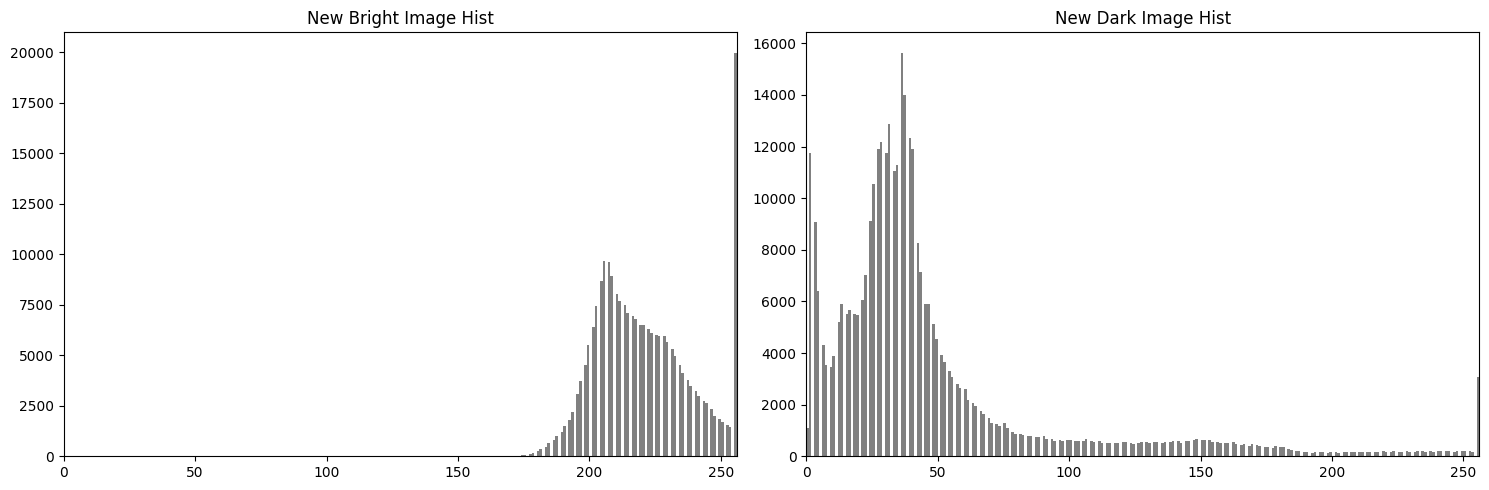
\includegraphics[width=0.9\linewidth]{images/image_257010.png} % هیستوگرام خروجی‌ها
    \caption{هیستوگرام تصاویر پس از انتقال افاین}
\end{subfigure}
\caption{نتایج اعمال فرمول ترکیبی $a \times I + b$. کنتراست و روشنایی به طرز چشمگیری بهبود یافته است.}
\label{fig:affine_transform}
\end{figure}

\begin{stepbox}
\field{۲. تحلیل نتایج بصری و بررسی هیستوگرام خروجی}{
همان‌طور که در نتایج بصری مشاهده می‌شود، اعمال این فرمول به طور همزمان مشکل رنگ‌پریدگی \texttt{BrightImage} و فشردگی و تاریکی \texttt{DarkImage} را برطرف کرده است. 

\textbf{پدیده \lr{Clipping} در کرانه‌ها:}
با دقت در هیستوگرام‌های خروجی، دو قله‌ی تند (\lr{Spike}) در مقادیر $0$ و $255$ دیده می‌شود. دلیل این امر آن است که با تحمیل انحراف معیار عریضِ $64$ به توزیع‌هایی که به شدت چوله (\lr{Skewed}) بوده‌اند، بخش‌هایی از دنباله‌ی هیستوگرام از بازه‌ی مجاز $[0, 255]$ خارج شده‌اند. تابع \lr{Clip} این مقادیر را روی صفر و ۲۵۵ فشرده کرده است. این یک \lr{Trade-off} مهندسی است: ما بخش کوچکی از اطلاعات در روشن‌ترین و تاریک‌ترین نقاط تصویر را فدا کردیم تا کنتراست کلی بافت‌ها و سوژه‌ی اصلی تصویر را به حداکثر برسانیم.
}
\end{stepbox}

\begin{notebox}[مقایسه با روش‌های دیگر]
هرچند این روش برای تصاویر با توزیع تک‌قله‌ای بسیار قدرتمند است، اما استفاده از آماره‌های سراسری (\lr{Global Statistics}) برای همه تصاویر ایده‌آل نیست. برای توزیع‌های پیچیده‌تر، نیاز به روش‌های غیرخطی توزیع احتمال مانند \lr{Histogram Equalization} داریم که در بخش‌های بعدی تمرین بررسی خواهند شد.
\end{notebox}